The next prototype, TRITIUM-IFIC 1, was designed to overcome the problems and limitations found in TRITIUM-IFIC 0. The main improvements were:

\begin{enumerate}

\item{} The fiber bundle was arranged straight to optimize the photon collection efficiency of the fibers.

\item{} A special fiber cleaning protocol, described in section \ref{subsec:CleaningProcess}, was applied to the fibers to improve the interfaces between fiber and tritiated water. This protocole produces a better wetting property of the fiber, which improves the photon collection efficiency of the scintillating fibers.

\item{} A Teflon vessel was used in the Tritium prototypes to improve the photon collection efficiency of the fibers, which is an intrinsic characteristic of the fiber that cannot be changed.

Teflon is a convenient material for its optical properties, specifically its reflection factor, which is very close to $100\%$ at the working wavelength. This means that the photons that escape from the fiber will hit the Teflon walls and go back to the scintillating fiber.

\end{enumerate}

The TRITIUM-IFIC 1 prototype consists of 64 straight scintillating fibers, of $20~\cm$ length, arranged within a Teflon structure in an $8\times 8$ square matrix, shown in Figure \ref{fig:TeflonStructureFibersTritiumIFIC1}.

\begin{figure}[h]
\centering
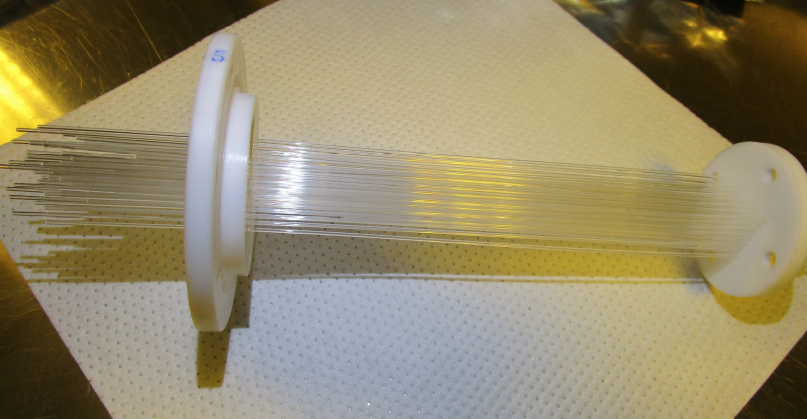
\includegraphics[scale=0.4]{5Prototypes/52PreliminarPrototypes/522TritiumIFIC1/FiberMatrixTeflonStructure.png}
\caption{Teflon structure used to arrange the fibers of TRITIUM-IFIC 1 prototype in a matrix of $8\cdot{}8$.\label{fig:TeflonStructureFibersTritiumIFIC1}}
\end{figure}
This structure is placed within a cylindrical Teflon vessel of $48~\mm$ diamenter and $200~\mm$ length, shown in Figure \ref{fig:TeflonVesselTritumIFIC1}. 

\begin{figure}
\centering
    \begin{subfigure}[b]{0.30\textwidth}
    \centering
    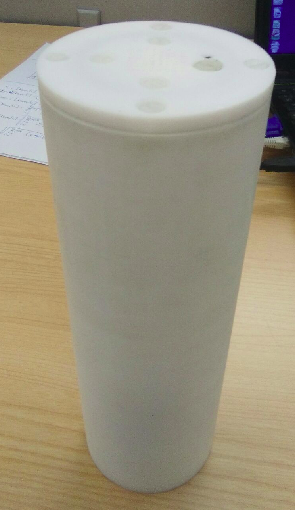
\includegraphics[width=\textwidth]{5Prototypes/52PreliminarPrototypes/522TritiumIFIC1/TeflonVesselTritiumIFIC1a.png}  
    \caption{\label{subfig:TeflonVesselTritumIFIC1a}}
    \end{subfigure}
    \hfill
    \begin{subfigure}[b]{0.45\textwidth}
    \centering
    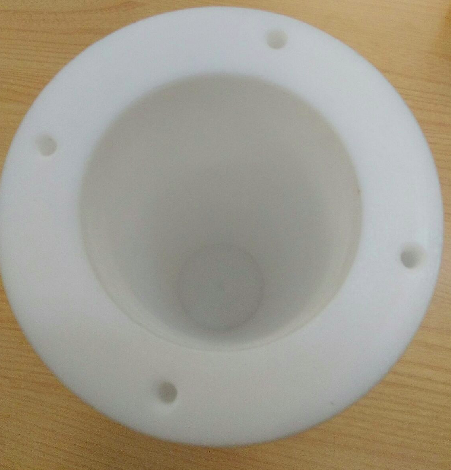
\includegraphics[width=\textwidth]{5Prototypes/52PreliminarPrototypes/522TritiumIFIC1/TeflonVesselTritiumIFIC1b.png}  
    \caption{\label{subfig:TeflonVesselTritumIFIC1b}}
    \end{subfigure}
 \caption{Teflon vessel of TRITIUM-IFIC 1 prototype.}
 \label{fig:TeflonVesselTritumIFIC1}
\end{figure}

The cleaning process, described in section \ref{subsec:CleaningProcess}, was applied to the fibers to achieve a better tritiated water-fiber interface. A PVC piece was used to attach the photosensor to the prototype and prevent external light from being read by photosensors. A general view of this prototype is shown in Figure \ref{fig:TritumIFIC1}.

\begin{figure}
\centering
    \begin{subfigure}[b]{0.40\textwidth}
    \centering
    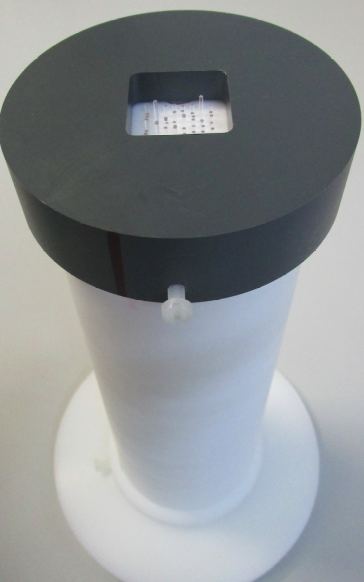
\includegraphics[width=\textwidth]{5Prototypes/52PreliminarPrototypes/522TritiumIFIC1/TritiumIFIC1a.png}  
    \caption{\label{subfig:TritumIFIC1a}}
    \end{subfigure}
    \hfill
    \begin{subfigure}[b]{0.40\textwidth}
    \centering
    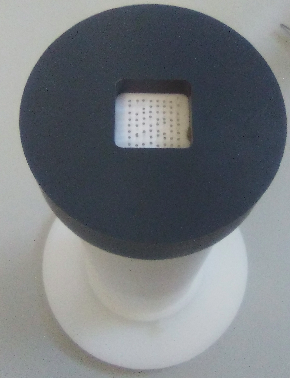
\includegraphics[width=\textwidth]{5Prototypes/52PreliminarPrototypes/522TritiumIFIC1/TritiumIFIC1b.png}  
    \caption{\label{subfig:TritumIFIC1b}}
    \end{subfigure}
 \caption{A general view of TRITIUM-IFIC 1 prototype.}
 \label{fig:TritumIFIC1}
\end{figure}

The prototype was read by a PMT R8520-460, from Hamamatsu Photonics company \cite{DataSheetPMTs} coupled directly to the fiber bundle using optical grease \cite{OpticalGrease}. The electronic circuit, shown in Figure \ref{fig:VoltageDividerCircuit}, was used to distribute the high voltage between the dynodes. The high voltage was $-800~\volt$, which corresponds to a quantum efficiency of $28.66\%$.

The signal from this PMT was acquired by the same electronic configuration used for the TRITIUM-IFIC 0 prototype, shown in Figure \ref{subfig:ElectronicConfiguraiton1PMT}. Unlike the first prototype, only one TRITIUM-IFIC 1 was built. In a first measurement, this prototype was filled with pure water ($118~\milli\liter$, uncertainty of $0.05\%$) and several background measurements were taken over a week. Then, it was emptied and refilled with $118~\milli\liter$ (uncertainty of $0.05\%$) of a tritiated water source of the same activity as the one used for TRITIUM-IFIC 0 prototype, $99.696~\kilo\becquerel/\liter$. The results of these measurements are presented in section \ref{subsec:ResultsTritiumIFIC1}, where they are compared to TRITIUM-IFIC 0 prototype results.

The signal and background energy spectra measured for this prototype are shown in Figure \ref{subfig:SignalBackgroundEnergySpectraTritiumIFIC1}. The difference between both energy spectra corresponds to the tritium energy spectrum, Figura \ref{subfig:TritiumEnergySpectraTritiumIFIC1}. The detection efficiency was quantified as in the previous section. The rate measured are given in Table \ref{tab:CountsPerSecondTRITIUMIFIC1}, where the tritium counts are obtained from the difference of signal and background spectra.

\begin{figure}
\centering
    \begin{subfigure}[b]{1\textwidth}
    \centering
    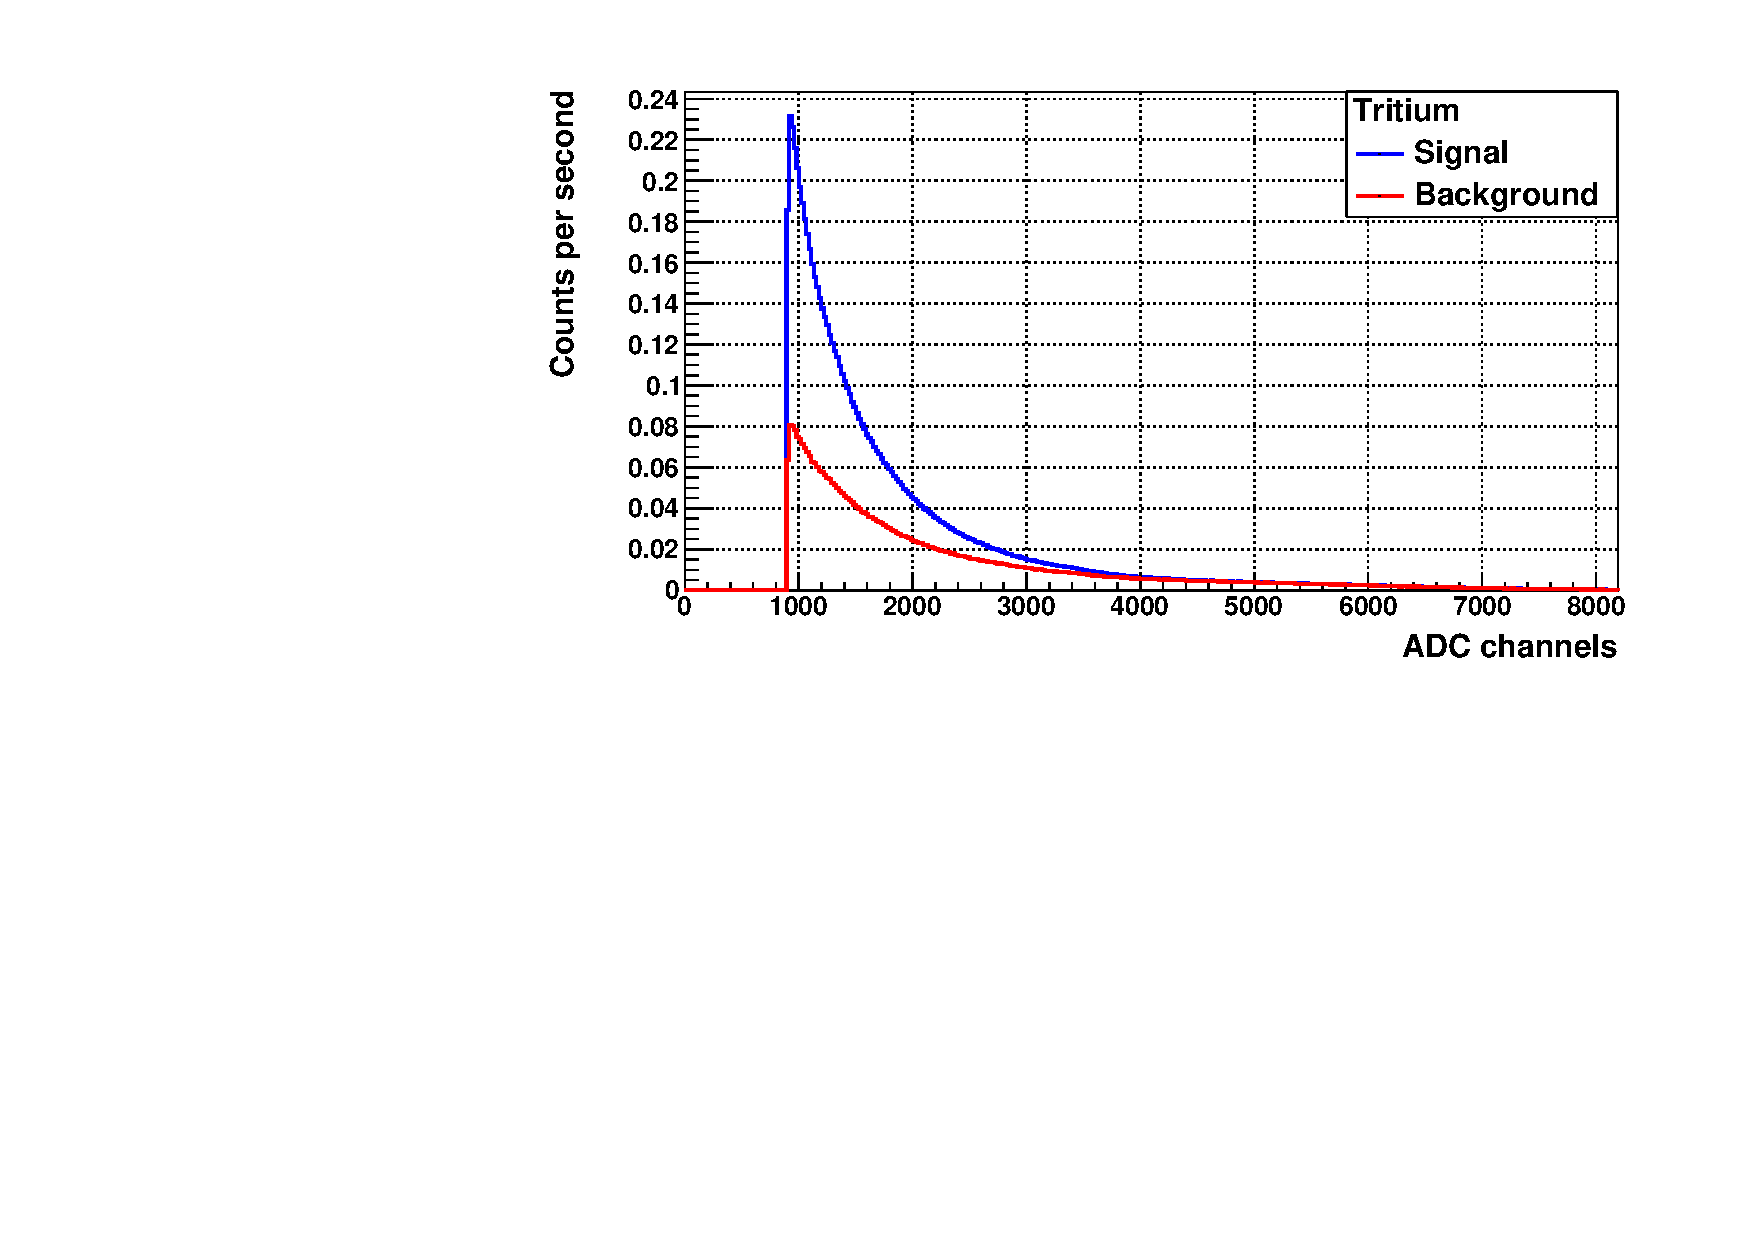
\includegraphics[width=\textwidth]{7ExperimentalResultsDetectors/71ExperimentalResultsLaboratory/712TRITIUMIFIC1/TritiumIFIC1Signals.pdf}  
    \caption{\label{subfig:SignalBackgroundEnergySpectraTritiumIFIC1}}
    \end{subfigure}
    \hfill
    \begin{subfigure}[b]{1\textwidth}
    \centering
    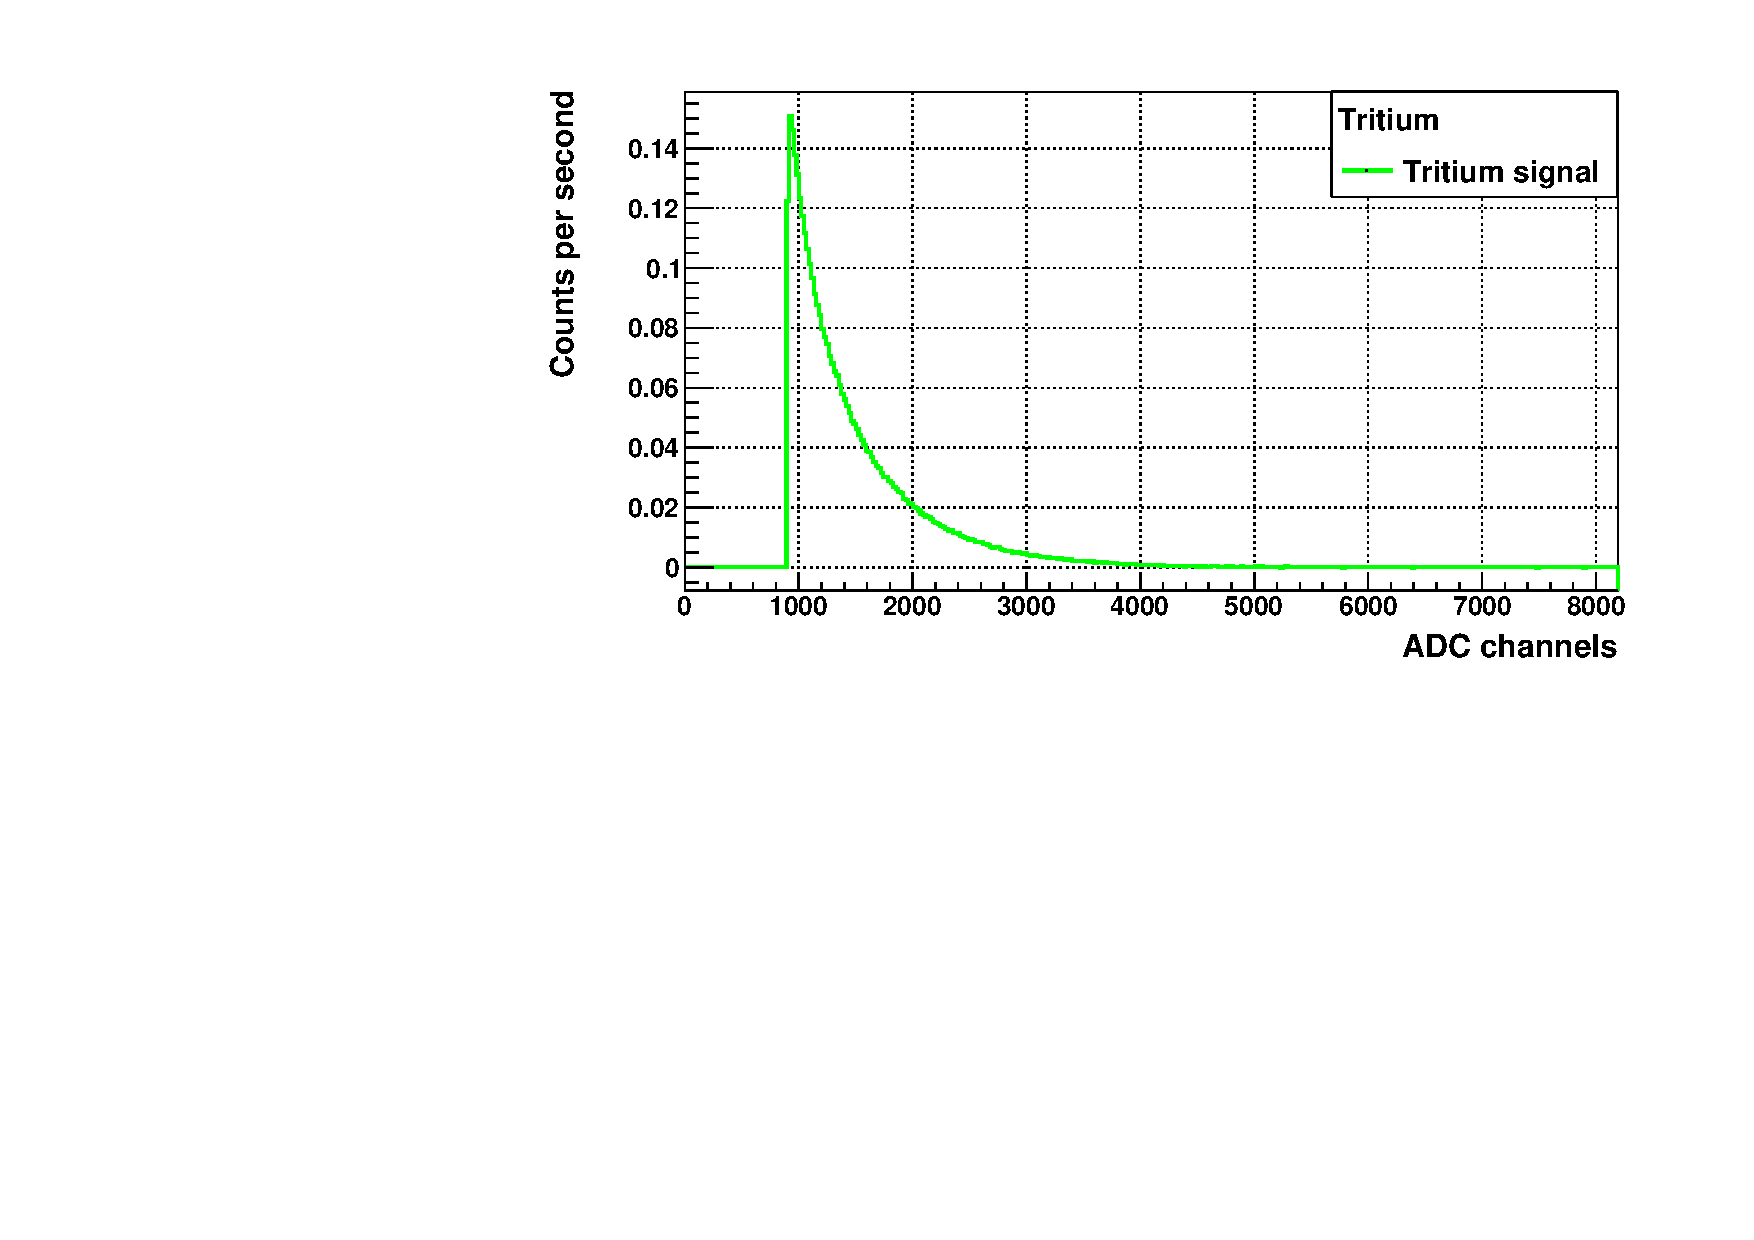
\includegraphics[width=\textwidth]{7ExperimentalResultsDetectors/71ExperimentalResultsLaboratory/712TRITIUMIFIC1/TritiumIFIC1Clear.pdf}  
    \caption{\label{subfig:TritiumEnergySpectraTritiumIFIC1}}
    \end{subfigure}
 \caption{Energy spectra measured with TRITIUM-IFIC 1 prototype. a) Signal and background energy spectra. b) Tritium energy spectrum.}
 \label{fig:EnergySpectraTRITIUMIFIC1}
\end{figure}

\begin{table}[htbp]
\centering{}%
\begin{tabular}{cc}
\toprule 
Spectrum & Counts/second \tabularnewline
\midrule
\midrule 
Signal prototype & $7.82 \pm 0.11$ \tabularnewline
Background prototype & $3.99 \pm 0.08$ \tabularnewline  
Tritium counts & $3.83 \pm 0.13$ \tabularnewline
\bottomrule
\end{tabular}
\caption{Counting rate obtained with the TRITIUM-IFIC 1 prototype.}
\label{tab:CountsPerSecondTRITIUMIFIC1}
\end{table}

The tritium detection efficiency obtained for TRITIUM-IFIC 1 is $(3.84 \pm 0.16)\cdot{} 10^{-2}~\liter\second^{-1}\kilo\becquerel^{-1}$. The efficiency obtained for this prototype is larger than that of TRITIUM-IFIC 0, as expected since this prototype has a larger active area. The specific efficiency obtained is $(9.56 \pm 0.40)\cdot{} 10^{-5}~\liter\second^{-1}\kilo\becquerel^{-1}\cm^{-2}$, which is a factor of ten better than that of TRITIUM-IFIC 0. Furthermore, compared to scintillating detectors developed in other experiments, table \ref{tab:PlasticScinTritium}, the efficiency of this prototype is very close to the best result, obtained by Singh, and the specific efficiency, which is the most relevant parameter to compare, is almost 5 times larger than that obtained by Hofstetter \cite{Hofstetter1, Hofstetter2}.